%%% Title:    Missing Data Stats Camp Course: MI Diagnostics
%%% Author:   Kyle M. Lang
%%% Created:  2017-SEP-12
%%% Modified: 2018-OCT-18

\documentclass{beamer}\usepackage[]{graphicx}\usepackage[]{color}
%% maxwidth is the original width if it is less than linewidth
%% otherwise use linewidth (to make sure the graphics do not exceed the margin)
\makeatletter
\def\maxwidth{ %
  \ifdim\Gin@nat@width>\linewidth
    \linewidth
  \else
    \Gin@nat@width
  \fi
}
\makeatother

\definecolor{fgcolor}{rgb}{0, 0, 0}
\newcommand{\hlnum}[1]{\textcolor[rgb]{0.69,0.494,0}{#1}}%
\newcommand{\hlstr}[1]{\textcolor[rgb]{0.749,0.012,0.012}{#1}}%
\newcommand{\hlcom}[1]{\textcolor[rgb]{0.514,0.506,0.514}{\textit{#1}}}%
\newcommand{\hlopt}[1]{\textcolor[rgb]{0,0,0}{#1}}%
\newcommand{\hlstd}[1]{\textcolor[rgb]{0,0,0}{#1}}%
\newcommand{\hlkwa}[1]{\textcolor[rgb]{0,0,0}{\textbf{#1}}}%
\newcommand{\hlkwb}[1]{\textcolor[rgb]{0,0.341,0.682}{#1}}%
\newcommand{\hlkwc}[1]{\textcolor[rgb]{0,0,0}{\textbf{#1}}}%
\newcommand{\hlkwd}[1]{\textcolor[rgb]{0.004,0.004,0.506}{#1}}%
\let\hlipl\hlkwb

\usepackage{framed}
\makeatletter
\newenvironment{kframe}{%
 \def\at@end@of@kframe{}%
 \ifinner\ifhmode%
  \def\at@end@of@kframe{\end{minipage}}%
  \begin{minipage}{\columnwidth}%
 \fi\fi%
 \def\FrameCommand##1{\hskip\@totalleftmargin \hskip-\fboxsep
 \colorbox{shadecolor}{##1}\hskip-\fboxsep
     % There is no \\@totalrightmargin, so:
     \hskip-\linewidth \hskip-\@totalleftmargin \hskip\columnwidth}%
 \MakeFramed {\advance\hsize-\width
   \@totalleftmargin\z@ \linewidth\hsize
   \@setminipage}}%
 {\par\unskip\endMakeFramed%
 \at@end@of@kframe}
\makeatother

\definecolor{shadecolor}{rgb}{.97, .97, .97}
\definecolor{messagecolor}{rgb}{0, 0, 0}
\definecolor{warningcolor}{rgb}{1, 0, 1}
\definecolor{errorcolor}{rgb}{1, 0, 0}
\newenvironment{knitrout}{}{} % an empty environment to be redefined in TeX

\usepackage{alltt}
\usetheme[%
  pageofpages          = of,
  bullet               = circle,
  titleline            = true,
  alternativetitlepage = true,
  titlepagelogo        = Logo3,
  watermark            = watermarkTiU,
  watermarkheight      = 100px,
  watermarkheightmult  = 4%
]{UVT}

\usepackage{graphicx}
\usepackage{booktabs}
\usepackage[natbibapa]{apacite}
\usepackage[libertine]{newtxmath}
\usepackage{fancybox}
\usepackage{caption}
\usepackage{upgreek}

\newcommand{\bup}{\boldsymbol{\betaup}}

%% Ensure styles of `blocks' (used in Definitions, Theorems etc.) follows the
%% UVT-style theme:
\setbeamercolor{block title}{fg = darkblue, bg = white}
\setbeamercolor{block body}{use = block title, bg = block title.bg}

%% Ensure TableOfContents is in UVT-style theme:
\setbeamercolor{section in toc}{fg = darkblue}

%% Don't number broken frames
\setbeamertemplate{frametitle continuation}{}

%% Don't label table captions:
\captionsetup{labelformat = empty}

\title{Multiple Imputation with Categorical Variables}
\subtitle{Stats Camp 2018: Missing Data Analysis}
\author{Kyle M. Lang}
\institute{Department of Methodology \& Statistics\\Tilburg University}
\date{19--21 October 2018}
\IfFileExists{upquote.sty}{\usepackage{upquote}}{}
\begin{document}

%------------------------------------------------------------------------------%



%------------------------------------------------------------------------------%

\begin{frame}[t,plain]
  
  \titlepage
  
\end{frame}

%------------------------------------------------------------------------------%

\begin{frame}{Outline}
  
  \begin{itemize}
  \item Discuss imputation diagnostics
    \vb
    \begin{itemize}
    \item Assessing imputation model convergence
      \vc
    \item Checking the imputations' plausibility
    \end{itemize}
    \vb
  \item Look at graphical and numerical options for both
  \end{itemize}
  
\end{frame}

%------------------------------------------------------------------------------%

\begin{frame}{Example Data}
  
  These data were analyzed by \citet{langEtAl:2009}.\\
  \begin{itemize}
  \item $N = 87$
  \item $V = 33$
  \item Variables assessing: 
    \begin{itemize}
    \item Perceptions of and Definitions of Racism
    \item Political Affiliation
    \item Support for Affirmative Action Policies
    \item Belief in meritocratic ideals
    \end{itemize}
    \vb
  \item Almost no missing data
    \begin{itemize}
    \item I've artificially imposed $30\%$ MAR missing data on all variables 
      (expect political affiliation) using political affiliation as the MAR 
      predictor.
    \end{itemize}
  \end{itemize}
  
\end{frame}

%------------------------------------------------------------------------------%
      
\begin{frame}{Imputation Diagnostics}

  After we run an MI routine, we need to make sure that the procedure has 
  performed as expected.\\
  \va
  Problems can arise to two different places:
  \begin{enumerate}
    \item The imputation model may fail to converge.
    \item The imputed values may not be plausible.
  \end{enumerate}
  \va 
  We need to examine our results to check for these problems.
  
\end{frame}

%------------------------------------------------------------------------------%

\begin{frame}{Imputation Model Convergence}
  
  The imputation model is usually estimated through some form of Bayesian 
  simulation.
  \vb
  \begin{itemize}
  \item Gibbs sampled parameters form a \emph{Markov Chain}.
    \begin{itemize}
    \item Each draw is dependent on only its immediate predecessor in the chain.
    \item $\theta^{(t)} | \theta^{(t - 1)} \perp \theta^{(t - j)} ~ \forall j > 1$
    \end{itemize}
    \vb
  \item Early elements of a Markov chain are similar to the starting values.
    \begin{itemize}
    \item Samples are poor approximations of the true posterior.
    \end{itemize}
    \vb
  \item We must let the sampler iterate for a while to allow the estimates time 
    to separate from their starting values.
    \begin{itemize}
    \item We call these initial iterations ``burn-in'' or ``warm-up'' 
      iterations.
    \end{itemize}
  \end{itemize}
  
\end{frame}

\watermarkoff %----------------------------------------------------------------%

\begin{frame}{Traceplots}
  
  Once converged, each sampled imputation model parameter should ``bounce'' 
  around an equilibrium point.
  \begin{itemize}
  \item The draws will never converge onto a single point.
  \item That would defeat the purpose of simulation-based inference.
  \end{itemize}
  
  \begin{columns}
    \begin{column}{0.5\textwidth}
      
\begin{knitrout}\footnotesize
\definecolor{shadecolor}{rgb}{0.878, 0.918, 0.933}\color{fgcolor}

{\centering 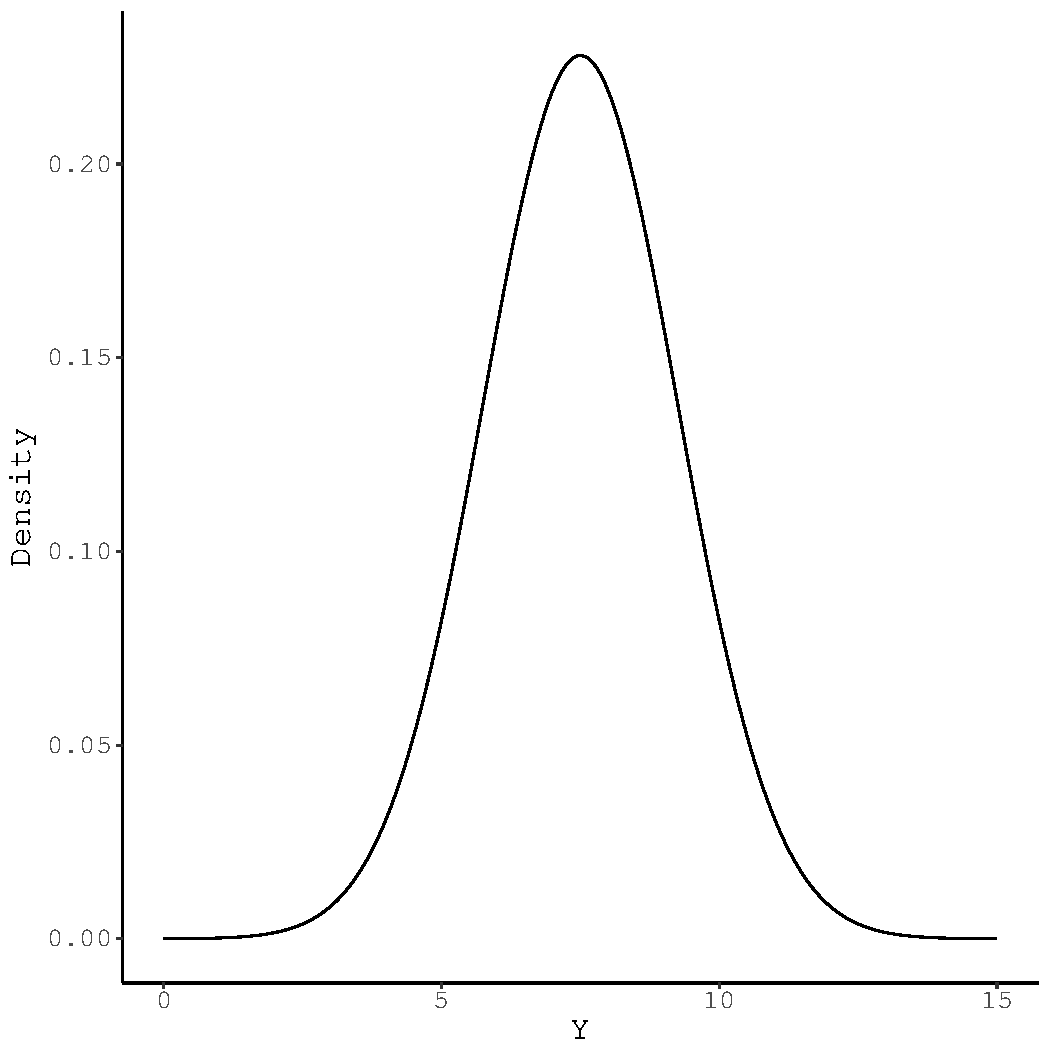
\includegraphics[width=0.95\linewidth]{figure/unnamed-chunk-1-1} 

}



\end{knitrout}

\end{column}

\begin{column}{0.5\textwidth}
  
\begin{knitrout}\footnotesize
\definecolor{shadecolor}{rgb}{0.878, 0.918, 0.933}\color{fgcolor}

{\centering 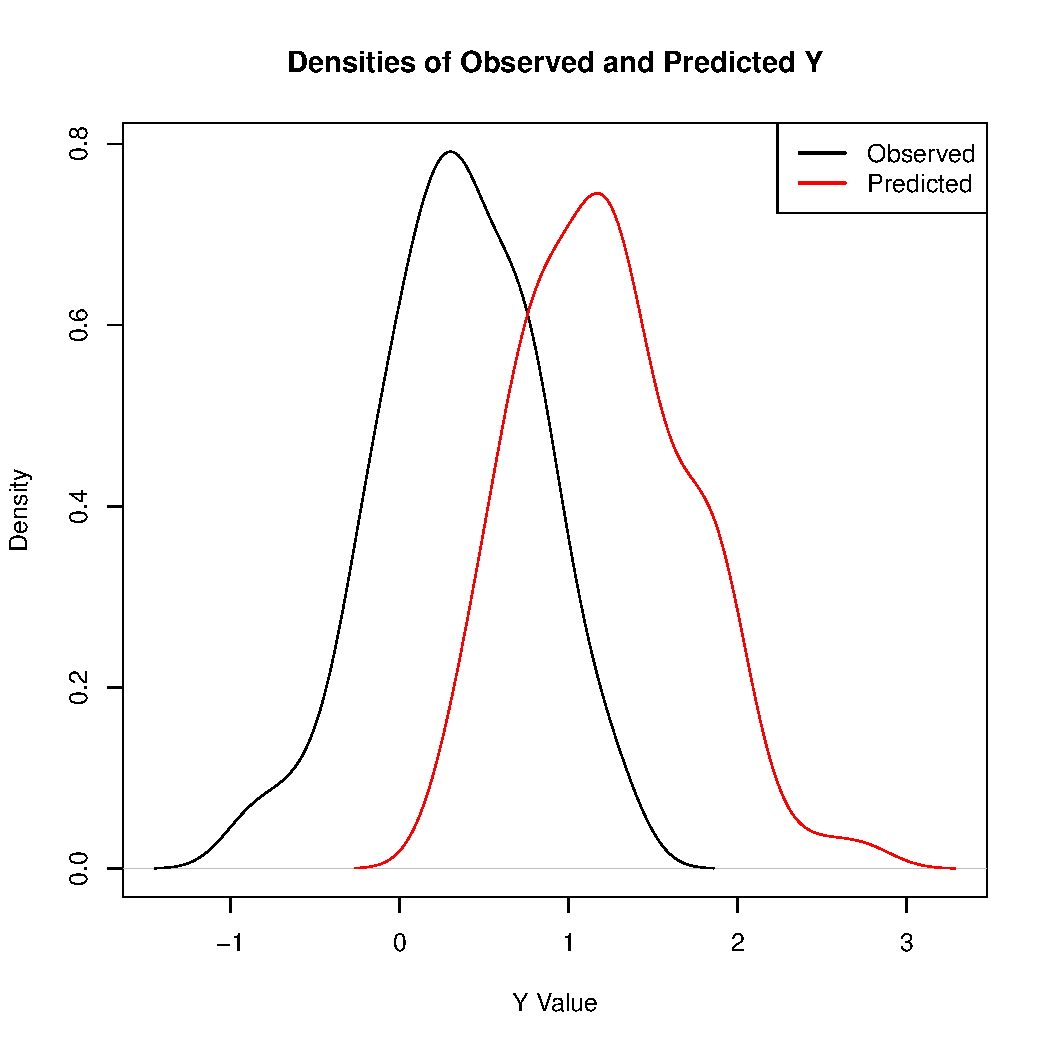
\includegraphics[width=0.95\linewidth]{figure/unnamed-chunk-2-1} 

}



\end{knitrout}

\end{column}
\end{columns}

\end{frame}

\watermarkon %-----------------------------------------------------------------%

\begin{frame}{Potential Scale Reduction Factor}
  
  Suppose we have two Markov chains for the same parameter.
  \vc 
  \begin{itemize}
  \item If these chains have converged, the average distance between any two
    points on separate chains should be the same as the average distance 
    between two points on the same chain.
    \vc
  \item The \emph{between-chain} variance should, on average, equal the 
    \emph{within-chain} variance.
  \end{itemize}
  \vc
  The \emph{Potential Scale Reduction Factor} $\widehat{R}$ quantifies this 
  concept:
  \begin{align*}
    \widehat{R} = \frac{\hat{\sigma}^2_{between}}{\hat{\sigma}^2_{within}}
  \end{align*}
  $\widehat{R}$ will approach 1.0 at convergence.
  \vc
  \begin{itemize}
  \item $\widehat{R} < $ 1.1 or 1.2 suggests acceptable convergence.
  \end{itemize}
  
\end{frame}

\watermarkoff %----------------------------------------------------------------%

\begin{frame}{Example: Potential Scale Reduction Factor}
   
\begin{knitrout}\footnotesize
\definecolor{shadecolor}{rgb}{0.878, 0.918, 0.933}\color{fgcolor}

{\centering 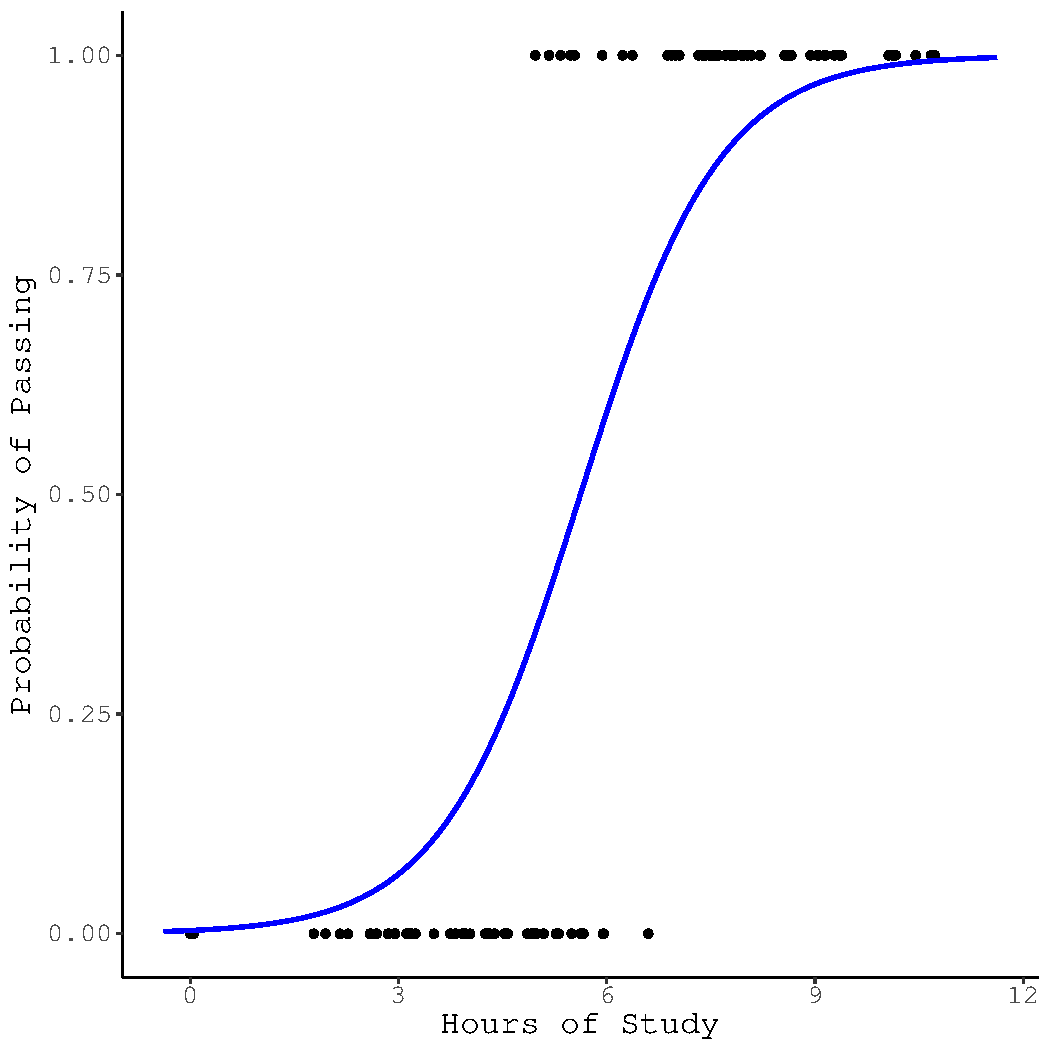
\includegraphics[width=0.65\linewidth]{figure/unnamed-chunk-3-1} 

}



\end{knitrout}

\end{frame}

%------------------------------------------------------------------------------%

\begin{frame}[fragile]{Example: Potential Scale Reduction Factor}
  
\begin{knitrout}\scriptsize
\definecolor{shadecolor}{rgb}{0.878, 0.918, 0.933}\color{fgcolor}\begin{kframe}
\begin{alltt}
\hlcom{## Create matrices of the full and burnt-in chains:}
\hlstd{iterMat}  \hlkwb{<-} \hlkwd{cbind}\hlstd{(chain1, chain2)}
\hlstd{burntMat} \hlkwb{<-} \hlstd{iterMat[}\hlnum{201} \hlopt{:} \hlnum{1000}\hlstd{, ]}

\hlcom{## Full Chain R-Hat:}
\hlstd{wVar1} \hlkwb{<-} \hlkwd{mean}\hlstd{(}\hlkwd{apply}\hlstd{(iterMat,} \hlnum{2}\hlstd{, var))}
\hlstd{bVar1} \hlkwb{<-} \hlkwd{mean}\hlstd{(}\hlkwd{apply}\hlstd{(iterMat,} \hlnum{1}\hlstd{, var))}
\hlstd{rHat1} \hlkwb{<-} \hlstd{bVar1} \hlopt{/} \hlstd{wVar1}
\hlstd{rHat1}
\end{alltt}
\begin{verbatim}
## [1] 1.682921
\end{verbatim}
\begin{alltt}
\hlcom{## Burnt-In R-Hat:}
\hlstd{wVar2} \hlkwb{<-} \hlkwd{mean}\hlstd{(}\hlkwd{apply}\hlstd{(burntMat,} \hlnum{2}\hlstd{, var))}
\hlstd{bVar2} \hlkwb{<-} \hlkwd{mean}\hlstd{(}\hlkwd{apply}\hlstd{(burntMat,} \hlnum{1}\hlstd{, var))}
\hlstd{rHat2} \hlkwb{<-} \hlstd{bVar2} \hlopt{/} \hlstd{wVar2}
\hlstd{rHat2}
\end{alltt}
\begin{verbatim}
## [1] 1.104803
\end{verbatim}
\end{kframe}
\end{knitrout}

\end{frame}

%------------------------------------------------------------------------------%

\begin{frame}[fragile, allowframebreaks]{More Imputation Model Convergence}
  
  A convergent imputation model will produce imputed values that
  fluctuate around an equilibrium point. 
  \vb
  \begin{itemize}
  \item Imputation model convergence can be assessed indirectly by
    looking at plots of the item-level sufficient statistics for each
    imputation.
  \end{itemize}
  \va
  This approach is automated for \textbf{mice} via \texttt{plot.mice()}.
  \va

\begin{knitrout}\footnotesize
\definecolor{shadecolor}{rgb}{0.878, 0.918, 0.933}\color{fgcolor}\begin{kframe}
\begin{alltt}
\hlstd{miceOut1} \hlkwb{<-} \hlkwd{readRDS}\hlstd{(}\hlkwd{paste0}\hlstd{(dataDir,} \hlstr{"miceOut1.rds"}\hlstd{))}
\hlkwd{plot}\hlstd{(miceOut1,} \hlkwd{c}\hlstd{(}\hlstr{"RIAE5"}\hlstd{,} \hlstr{"NORI4"}\hlstd{,} \hlstr{"POLICY2"}\hlstd{))}
\end{alltt}
\end{kframe}

{\centering 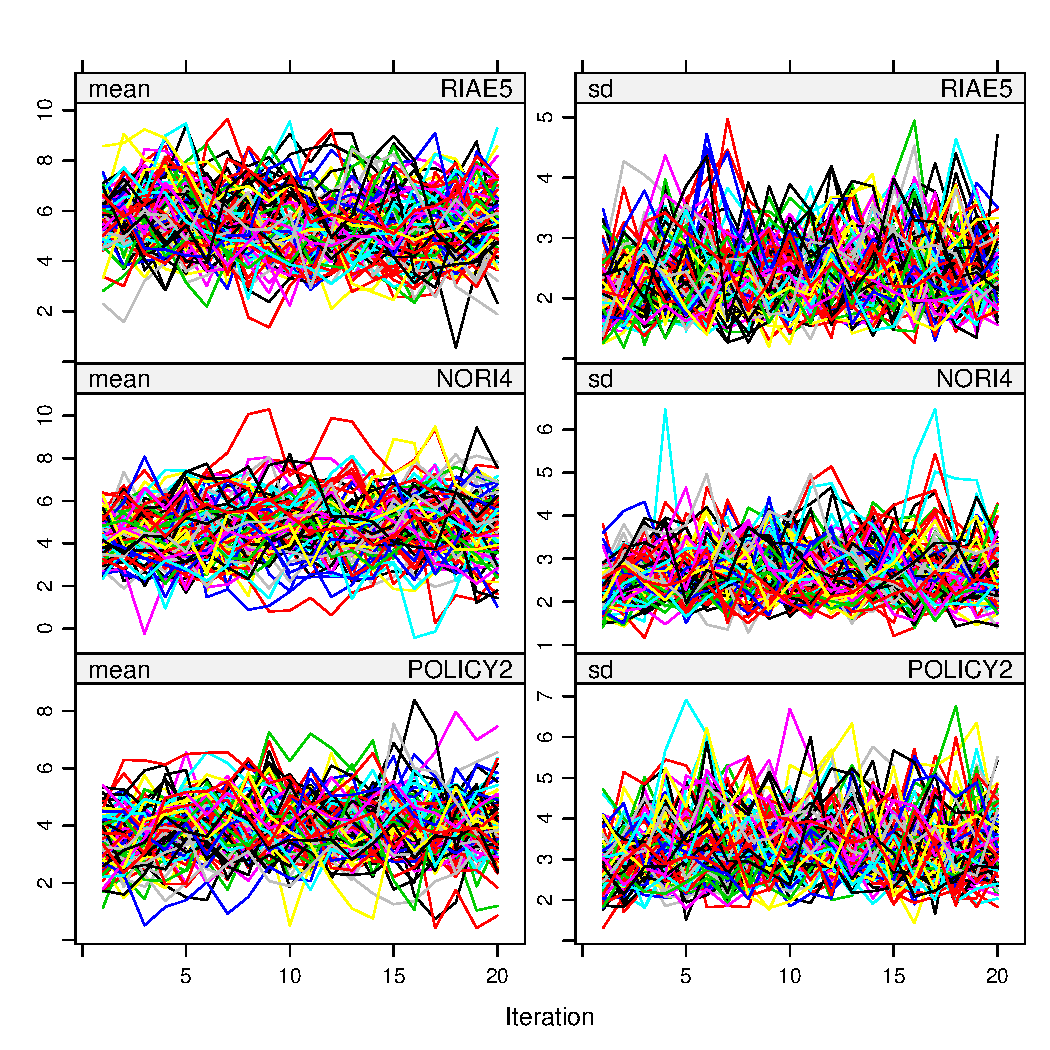
\includegraphics[width=0.65\linewidth]{figure/unnamed-chunk-5-1} 

}



\end{knitrout}

\end{frame}

\watermarkon %-----------------------------------------------------------------%

\begin{frame}{Imputed Value Plausibility}
  
  We need to ensure that the imputations are sensible.
  \vc
  \begin{itemize}
  \item Imputed values shouldn't be \emph{too} dissimilar from their observed 
    counterparts.
    \begin{itemize}
    \item What constitutes \emph{too} much dissimilarity is subjective and 
      problem-specific.
    \end{itemize}
  \end{itemize}
  \vb
  We can assess dissimilarity graphically or through summary statistics.
  \vc
  \begin{itemize}
  \item Out-of-bounds values for the imputations are perfectly acceptable.
    \begin{itemize}
    \item MI is \emph{NOT} designed to maintain the range.
    \item We don't want wildly extreme values, though.
    \end{itemize}
    \vc
  \item The means of the observed and imputed components of each variable 
    shouldn't differ too much.
    \begin{itemize}
    \item Again, how much is \emph{too} much is subjective.
    \end{itemize}
  \end{itemize}
  
\end{frame}

\watermarkoff %----------------------------------------------------------------%

\begin{frame}[fragile]{Numeric Imputation Checks}
  


\begin{knitrout}\footnotesize
\definecolor{shadecolor}{rgb}{0.878, 0.918, 0.933}\color{fgcolor}\begin{kframe}
\begin{alltt}
\hlstd{rawMeans} \hlkwb{<-} \hlkwd{colMeans}\hlstd{(missData,} \hlkwc{na.rm} \hlstd{=} \hlnum{TRUE}\hlstd{)}
\hlstd{impMeans} \hlkwb{<-} \hlkwd{colMeans}\hlstd{(}\hlkwd{do.call}\hlstd{(}\hlstr{"rbind"}\hlstd{, impList))}

\hlstd{rawSds} \hlkwb{<-} \hlkwd{apply}\hlstd{(missData,} \hlnum{2}\hlstd{, sd,} \hlkwc{na.rm} \hlstd{=} \hlnum{TRUE}\hlstd{)}
\hlstd{sdList} \hlkwb{<-} \hlkwd{lapply}\hlstd{(impList,} \hlkwa{function}\hlstd{(}\hlkwc{x}\hlstd{)} \hlkwd{sapply}\hlstd{(x,} \hlkwc{FUN} \hlstd{= sd))}
\hlstd{impSds} \hlkwb{<-} \hlkwd{colMeans}\hlstd{(}\hlkwd{do.call}\hlstd{(rbind, sdList))}

\hlstd{rawRanges} \hlkwb{<-} \hlkwd{apply}\hlstd{(missData,} \hlnum{2}\hlstd{, range,} \hlkwc{na.rm} \hlstd{=} \hlnum{TRUE}\hlstd{)}
\hlstd{impRanges} \hlkwb{<-} \hlkwd{sapply}\hlstd{(}\hlkwd{do.call}\hlstd{(}\hlstr{"rbind"}\hlstd{, impList), range)}
\end{alltt}
\end{kframe}
\end{knitrout}

\end{frame}

%------------------------------------------------------------------------------%

\begin{frame}[fragile, allowframebreaks]{Numeric Imputation Checks}

\begin{knitrout}\footnotesize
\definecolor{shadecolor}{rgb}{0.878, 0.918, 0.933}\color{fgcolor}\begin{kframe}
\begin{alltt}
\hlkwd{round}\hlstd{(rawMeans[}\hlnum{1} \hlopt{:} \hlnum{5}\hlstd{],} \hlnum{3}\hlstd{)}
\end{alltt}
\begin{verbatim}
## RIAE2 RIAE3 RIAE7 RIAE8 RIAE9 
## 3.677 3.108 3.774 3.092 3.726
\end{verbatim}
\begin{alltt}
\hlkwd{round}\hlstd{(impMeans[}\hlnum{1} \hlopt{:} \hlnum{5}\hlstd{],} \hlnum{3}\hlstd{)}
\end{alltt}
\begin{verbatim}
## RIAE2 RIAE3 RIAE7 RIAE8 RIAE9 
## 3.697 3.122 3.340 3.134 3.010
\end{verbatim}
\end{kframe}
\end{knitrout}

\pagebreak

\begin{knitrout}\footnotesize
\definecolor{shadecolor}{rgb}{0.878, 0.918, 0.933}\color{fgcolor}\begin{kframe}
\begin{alltt}
\hlkwd{round}\hlstd{(rawSds[}\hlnum{1} \hlopt{:} \hlnum{5}\hlstd{],} \hlnum{3}\hlstd{)}
\end{alltt}
\begin{verbatim}
## RIAE2 RIAE3 RIAE7 RIAE8 RIAE9 
## 1.696 1.522 2.060 1.693 1.700
\end{verbatim}
\begin{alltt}
\hlkwd{round}\hlstd{(impSds[}\hlnum{1} \hlopt{:} \hlnum{5}\hlstd{],} \hlnum{3}\hlstd{)}
\end{alltt}
\begin{verbatim}
## RIAE2 RIAE3 RIAE7 RIAE8 RIAE9 
## 2.223 1.906 2.917 2.157 2.283
\end{verbatim}
\end{kframe}
\end{knitrout}

\pagebreak

\begin{knitrout}\footnotesize
\definecolor{shadecolor}{rgb}{0.878, 0.918, 0.933}\color{fgcolor}\begin{kframe}
\begin{alltt}
\hlkwd{round}\hlstd{(rawRanges[ ,} \hlnum{1} \hlopt{:} \hlnum{5}\hlstd{],} \hlnum{3}\hlstd{)}
\end{alltt}
\begin{verbatim}
##      RIAE2 RIAE3 RIAE7 RIAE8 RIAE9
## [1,]     1     1     1     1     1
## [2,]     7     6     7     7     7
\end{verbatim}
\begin{alltt}
\hlkwd{round}\hlstd{(impRanges[ ,} \hlnum{1} \hlopt{:} \hlnum{5}\hlstd{],} \hlnum{3}\hlstd{)}
\end{alltt}
\begin{verbatim}
##       RIAE2  RIAE3   RIAE7  RIAE8   RIAE9
## [1,] -7.819 -8.486 -17.790 -9.473 -10.184
## [2,] 21.724 15.941  15.869 16.551  11.201
\end{verbatim}
\end{kframe}
\end{knitrout}

\end{frame}

%------------------------------------------------------------------------------%

\begin{frame}[fragile]{Graphical Imputation Checks}

\begin{knitrout}\scriptsize
\definecolor{shadecolor}{rgb}{0.878, 0.918, 0.933}\color{fgcolor}\begin{kframe}
\begin{alltt}
\hlcom{## Overlaid density plots of imputed vs. observed values:}
\hlkwd{densityplot}\hlstd{(miceOut1,} \hlkwc{data} \hlstd{=} \hlopt{~}\hlstd{RIAE5} \hlopt{+} \hlstd{NORI4} \hlopt{+} \hlstd{WPRIV7,}
            \hlkwc{layout} \hlstd{=} \hlkwd{c}\hlstd{(}\hlnum{3}\hlstd{,} \hlnum{1}\hlstd{))}
\end{alltt}
\end{kframe}

{\centering 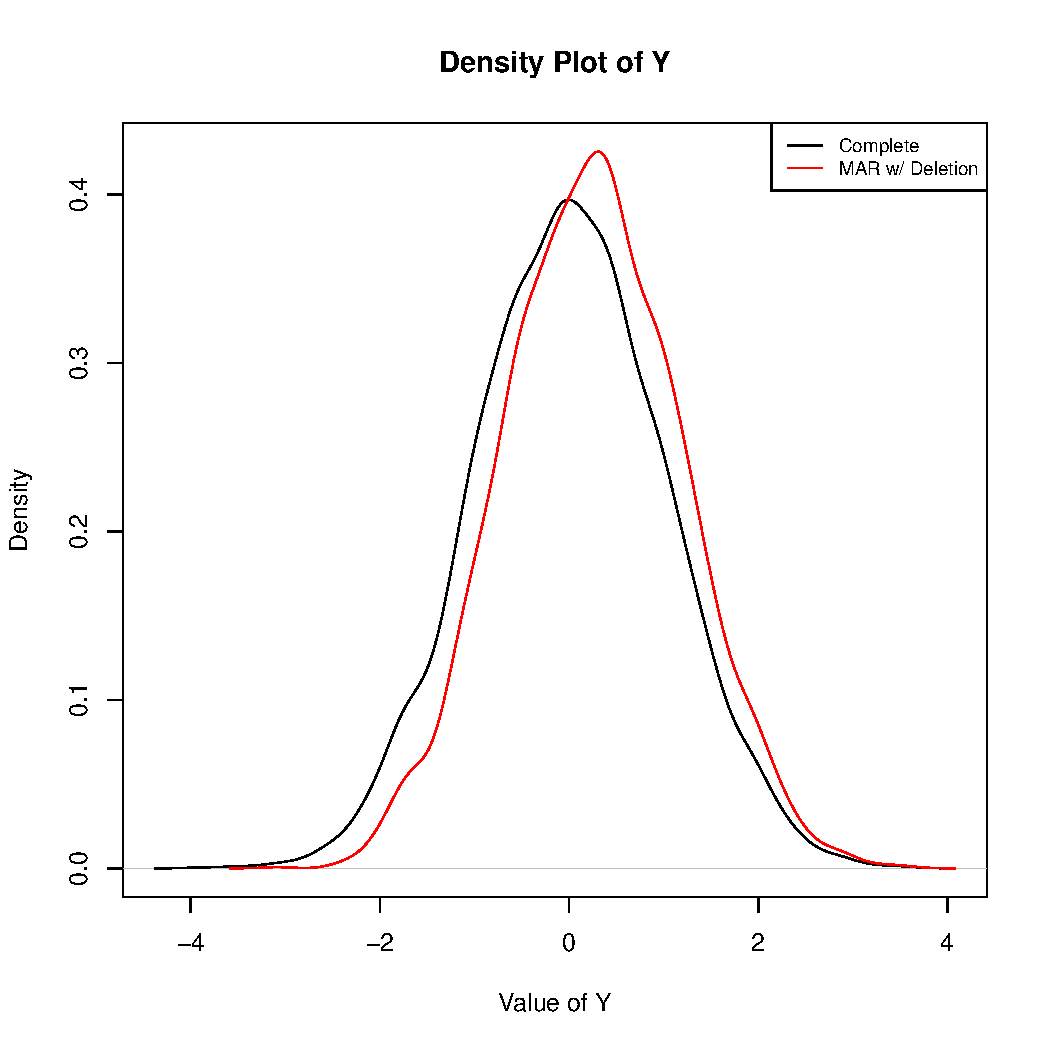
\includegraphics[width=0.65\linewidth,height=0.65\textheight]{figure/unnamed-chunk-11-1} 

}



\end{knitrout}
     
\end{frame}

%------------------------------------------------------------------------------%

\begin{frame}[fragile]{Graphical Imputation Checks}

\begin{knitrout}\scriptsize
\definecolor{shadecolor}{rgb}{0.878, 0.918, 0.933}\color{fgcolor}\begin{kframe}
\begin{alltt}
\hlcom{## Scatterplots of imputed vs. observed values:}
\hlkwd{stripplot}\hlstd{(miceOut1,} \hlkwc{data} \hlstd{= RIAE5} \hlopt{+} \hlstd{NORI4} \hlopt{+} \hlstd{WPRIV7} \hlopt{~} \hlstd{.imp,}
          \hlkwc{layout} \hlstd{=} \hlkwd{c}\hlstd{(}\hlnum{3}\hlstd{,} \hlnum{1}\hlstd{))}
\end{alltt}
\end{kframe}

{\centering 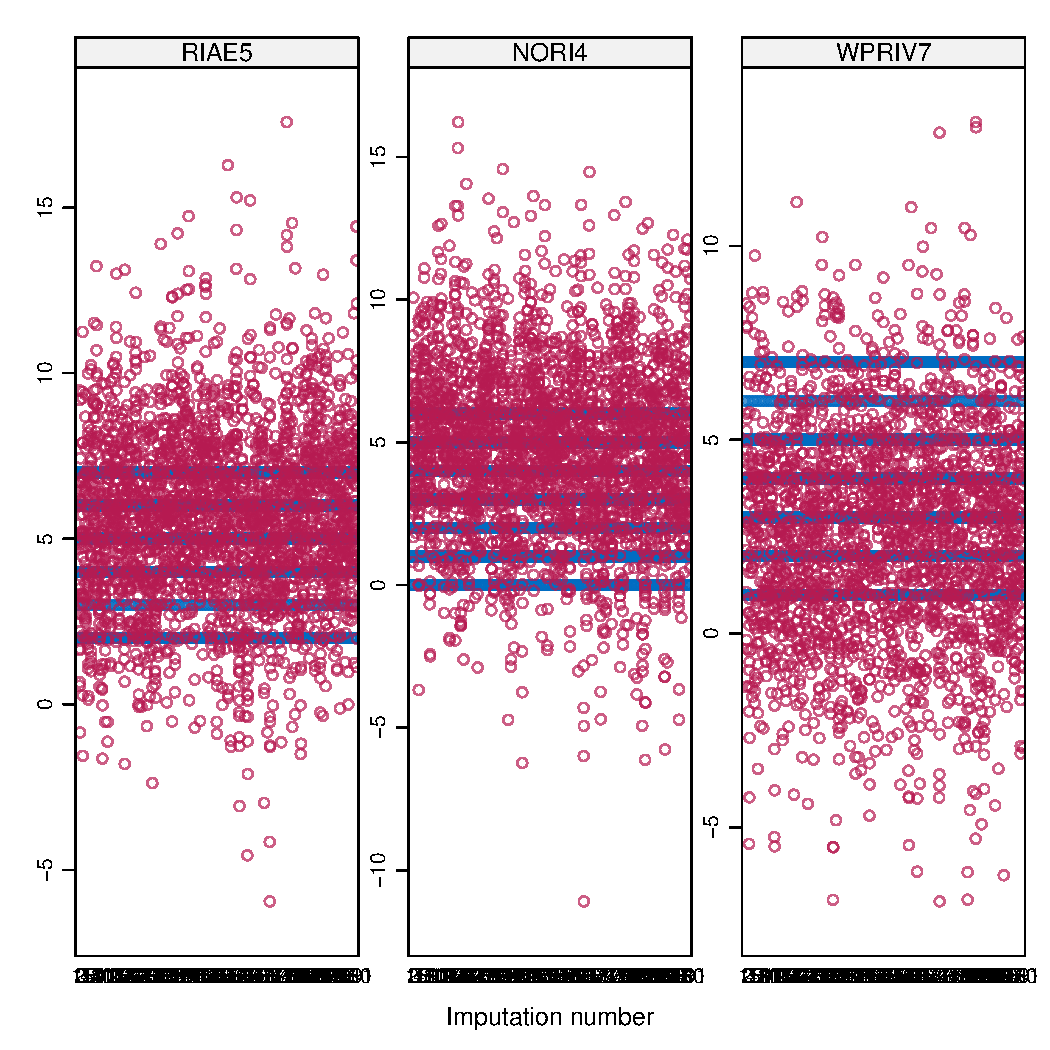
\includegraphics[width=0.65\linewidth,height=0.65\textheight]{figure/unnamed-chunk-12-1} 

}



\end{knitrout}

\end{frame}

%------------------------------------------------------------------------------%

\begin{frame}[fragile, allowframebreaks]{Graphical Imputation Checks}
    
  We can use the \texttt{plotImps} function from the \textbf{SURF} package to 
  generate overlaid density plots for arbitrary lists of imputed data.
  
\begin{knitrout}\footnotesize
\definecolor{shadecolor}{rgb}{0.878, 0.918, 0.933}\color{fgcolor}\begin{kframe}
\begin{alltt}
\hlcom{## Overlaid density plots of imputed vs. observed values:}
\hlkwd{par}\hlstd{(}\hlkwc{mfrow} \hlstd{=} \hlkwd{c}\hlstd{(}\hlnum{1}\hlstd{,} \hlnum{3}\hlstd{),} \hlkwc{cex.main} \hlstd{=} \hlnum{0.9}\hlstd{)}

\hlstd{rMat}                 \hlkwb{<-} \hlkwd{is.na}\hlstd{(miceOut1}\hlopt{$}\hlstd{data)}
\hlstd{type}                 \hlkwb{<-} \hlstd{miceOut1}\hlopt{$}\hlstd{method}
\hlstd{type[type} \hlopt{==} \hlstr{"norm"}\hlstd{]} \hlkwb{<-} \hlstr{"con"}

\hlkwd{plotImps}\hlstd{(}\hlkwc{impList}   \hlstd{= impList,}
         \hlkwc{rMat}      \hlstd{= rMat,}
         \hlkwc{typeVec}   \hlstd{= type,}
         \hlkwc{targetVar} \hlstd{=} \hlkwd{c}\hlstd{(}\hlstr{"RIAE5"}\hlstd{,} \hlstr{"NORI4"}\hlstd{,} \hlstr{"WPRIV7"}\hlstd{))}
\end{alltt}
\end{kframe}

{\centering 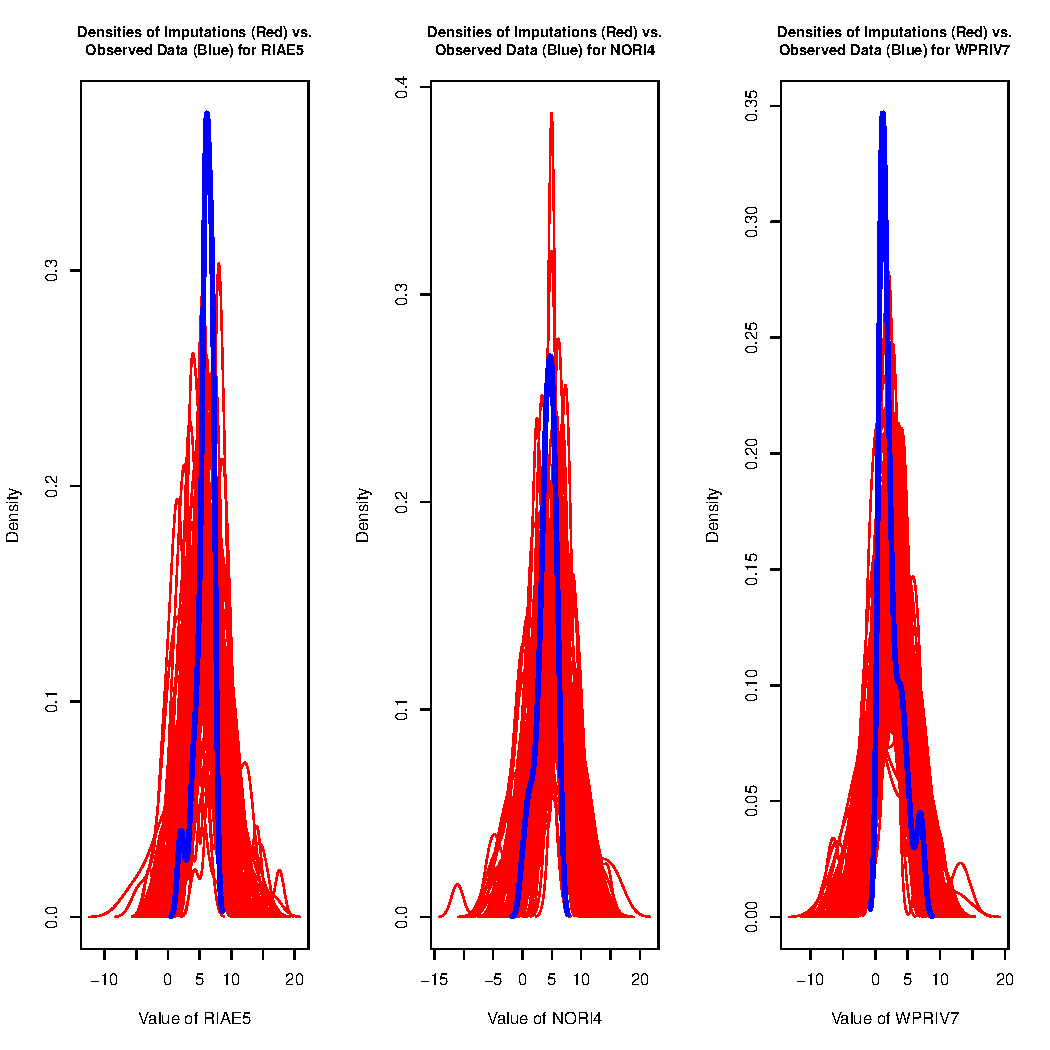
\includegraphics[width=0.65\linewidth]{figure/unnamed-chunk-13-1} 

}



\end{knitrout}

\end{frame}

\watermarkon %----------------------------------------------------------------%

\begin{frame}{References}

  \bibliographystyle{apacite}
  \bibliography{../../../literature/bibtexFiles/appliedRefs.bib}

\end{frame}

%------------------------------------------------------------------------------%

\end{document}
